% EQCCTPro draft — Overleaf-ready main file
% Upload: main.tex, body.tex, supplement.tex, and a folder "figures/" with assets from docs/figures/
\documentclass[11pt]{article}

\usepackage[T1]{fontenc}
\usepackage[utf8]{inputenc}
\usepackage{lmodern}
\usepackage[margin=1in]{geometry}
\usepackage{amsmath,amssymb}
\usepackage{graphicx}
\usepackage{booktabs}
\usepackage{multirow}
\usepackage{float}
\usepackage{caption}
\captionsetup{font=small,labelfont=bf}
\usepackage{pdflscape}
\usepackage{rotating}
\usepackage[hidelinks,unicode]{hyperref}
\usepackage{url}
\usepackage{microtype}
\usepackage{float}

\graphicspath{{figures/}}

\title{RAPID: A Generalized High-Performance Parallelization Framework for Real-Time Deep Learning Seismic Phase Picking}
\author{Author One \\ University of Texas at Austin \and Author Two \\ University of Texas at Austin}
\date{\today}

\begin{document}
\maketitle

\begin{abstract}
Deep learning has transformed seismic phase picking, yet deploying these models at network scale in real time remains an unresolved engineering challenge. While unified libraries such as SeisBench excel at high-throughput offline batch inference, these methods are ill-suited for continuous monitoring, where waveforms arrive asynchronously from individual stations and cannot be held in memory until a full batch is assembled. The naive alternative, dispatching each station as an independent parallel task, forces repeated framework initialization for every waveform, inflating wall times and consuming much of the available compute time budget unless concurrency and hardware are tuned carefully. To resolve this, we introduce \textbf{RAPID (Resource-Aware Parallel Inference Dispatcher)}, a generalized orchestration framework that implements two task parallelization strategies: \textbf{Ripper}, an ephemeral task-based approach, and \textbf{Model-Actor}, which keeps persistent inference instances loaded in memory across an entire processing window. We benchmarked RAPID across five deep learning phase pickers (PhaseNet, PhaseNetLight, EQTransformer, EQTransformer-NonConservative, and EQCCT) using 228 three-component 60-second waveforms from the Texas Seismological Network under various hardware constraints that reflect real operational deployment scenarios. Across all configurations, the Model-Actor strategy achieved real-time processing, reducing processing time by roughly \textbf{50--87\%} relative to the best Ripper totals at 228 stations for the same model--hardware pairings. These results show that the dominant bottleneck in network-scale DL picking is not raw inference complexity but orchestration overhead, and that persistent-actor lifecycle management delivers substantially faster totals and larger headroom under the 30-second target than even the best tuned ephemeral-task baseline.
\end{abstract}

\section{Introduction}

Accurate and timely identification of seismic phase arrivals is fundamental to earthquake monitoring. For decades, seismic networks have, and continue to rely on, energy-ratio algorithms, primarily the Short-Term Average/Long-Term Average (STA/LTA), to automate event detection. While computationally inexpensive, these algorithms are sensitive to background noise, requiring station-specific tuning, and often leading to high rates of false-positives in complex noise environments.

Over the past decade, deep learning (DL) has emerged as a powerful alternative. Models such as PhaseNet (Zhu \& Beroza, 2018), EQTransformer (Mousavi et al., 2020), and EQCCT (Saad et al., 2023) consistently outperform traditional picking methods in both precision and recall, particularly in low signal-to-noise conditions. SeisBench (Woollam et al., 2022) has consolidated many of these models into a unified interface along with several datasets (Münchmeyer et al., 2022), establishing itself as the standard library for DL-based seismic phase-picking research.

This progress has naturally led researchers to seek to incorporate these pickers into production workflows with real-time operations in mind. We define \emph{real-time processing} as returning picks for a full station selection within 30 seconds of a 60-second processing window. Chen, Savvaidis, et al. (2024) describe a near real-time workflow with EQCCT in SeisComP as their main picking algorithm, together with association, relocation, and catalog quality control; their evaluation foregrounds catalog quality and analyst workflow rather than a tight, network-scale bound on picking latency alone. Yeck et al. (2020) sketch a related deployment at NEIC with compact CNNs that refine STA/LTA detections before association; their reported timings use replayed automatic product streams, which—like our own offline waveforms benchmark—is appropriate for characterizing that pipeline’s throughput, but it still does not answer how large-window DL pickers behave when hundreds of stations must finish within a strict local compute budget. Sheen et al. (2023) replace traditional (non-DL) single-channel Earthworm pickers with a module that walks 30 s windows every second on WAVE\_RING using ordinary Earthworm utilities: fast for that ring-based path, but still focused on classical detectors rather than on coordinating regional DL pickers over many stations at once.

These systems are instructive, yet none solves our core question: \textbf{how to run today’s most widely used DL pickers when restrictive CPU, GPU, memory, and timing constraints are presented.} We therefore started with SeisBench, where many of the most widely used models are already easily accessible, and ask what available solutions on the platform enable real-time processing once station count and the 30-second window are jointly constrained by hardware limitations.

Currently, SeisBench supports two primary waveform processing modes. The first, \emph{offline batch mode}, processes waveforms in a single \texttt{annotate()} call. This method uses internal batching to achieve sub-second runtimes for entire networks (0.22–1.22 s for 228 stations, Table 1). While highly effective for post-event analysis, it is incompatible with real-time monitoring. Operationally, waveforms arrive asynchronously from individual stations due to factors such as network latency or power failures. As a result, incoming waveforms cannot be held in memory until a full batch is assembled because the processing window will continue to advance forward in time.

The second mode, \emph{per-station streaming}, uses the \texttt{classify()} method to process one waveform at a time. This method windows the incoming trace, runs a forward pass, and extracts phase arrivals. Since the model remains in memory between calls, no per-station reinitialization cost is paid. For the four SeisBench-integrated architectures tested, sequential processing of 228 stations requires 1.43–33.70 s. While these times might seem sufficient, \texttt{classify()} has four structural limitations:

(1) \textbf{Hardware non-scalability}. Because \texttt{classify()} processes stations sequentially, adding more CPU cores or GPUs does not improve throughput. Runtime remains limited by the performance of a single model instance.

(2) \textbf{Operational scale failure}. Scaling to even larger network sizes, PhaseNet running on a single CPU reaches 35.85 s for 250 stations (TexNet) and 80.23 s for 580 stations (NCSN), already exceeding real-time deadlines.

(3) \textbf{Shared inference budget}. The 30-second real-time compute window must also accommodate data quality checks, phase association, and alert dispatch. A 2-second margin is insufficient for operational stability.

(4) \textbf{Registry limitations}. Models not yet integrated into SeisBench, such as EQCCT or custom institutional pickers, lack a \texttt{classify()} path, forcing networks to find other multi-waveform processing alternatives.

While parallelization is the intuitive remedy for these sequential processing constraints, treating each station as a separate parallel task forces the machine learning framework to re-initialize for every station. On our hardware that cost dominates runtimes, as will be discussed later, leaving little margin for association, quality control, and dispatch.

To address these issues, we introduce \textbf{RAPID (Resource-Aware Parallel Inference Dispatcher)}, a generalized, resource-aware parallelization framework for seismic phase picking. RAPID is designed to complement SeisBench by using its native \texttt{from\_pretrained()}, \texttt{annotate()}, and \texttt{classify()} interfaces while providing the necessary orchestration for real-time operations. We implement two parallelization strategies: \textbf{Model-Actor} (persistent instances) and \textbf{Ripper} (ephemeral tasks). We benchmarked these across five pickers and two hardware configurations. The Model-Actor method reduced total runtimes by roughly 50–87\% compared with the best Ripper totals at 228 stations for the same model–device pairs, demonstrating that persistent-actor orchestration yields faster end-to-end times and more comfortable real-time margin than tuned ephemeral-task Ripper on real-world network workloads.

\section{Methodology}

The methodology is organized as follows: dataset and workload simulation (\S2.1), model selection (\S2.2), hardware environment and resource control (\S2.3), orchestration strategies (\S2.4), performance metrics (\S2.5), and study protocol (\S2.6).

\subsection{Dataset and Workload Simulation}

To evaluate our proposed parallelization strategies that would enable real-time seismic processing, we used data from the Texas Seismological Network (TexNet, Savvaidis et al., 2019) to simulate realistic network-scale inputs. From TexNet's 250 stations, we retrieved 228 unique three-component (3-C) 60-second waveforms, sampled at 100 Hz, for an M4.29 event that occurred on 26 January 2026 in West Texas. The 60-second window was chosen as it is the minimum input requirement for EQCCT (Saad et al., 2023) as well as matches TexNet's standard operational interval. Although models such as PhaseNet can accept shorter window durations, we used a uniform one-minute input across all models to ensure a fair comparison of orchestration performance under identical workload conditions. We were only able to retrieve 228 station records for that given time window, as the remaining 22 stations were either delayed, down, or in maintenance at the time, further reflecting the issues that come with real time network processing.

Waveforms were pre-downloaded as miniSEED files to exclude network latency from the benchmark. During execution, waveforms are converted to NumPy arrays and stored in memory-resident Python dictionaries. This design isolates inference and orchestration costs from disk I/O. A 1-45 Hz bandpass filter was applied to all data during inference as a standard preprocessing step for high-frequency phase identification.

\subsection{Model Selection}

To demonstrate that the primary performance bottleneck is overhead rather than model architecture, we benchmarked the strategies across five model solutions:

\begin{enumerate}
\item \textbf{PhaseNet} (U-Net; Zhu \& Beroza, 2018),
\item \textbf{PhaseNetLight} (Optimized PhaseNet; Woollam et al., 2022)
\item \textbf{EQTransformer} (Attention-based; Mousavi et al., 2020)
\item \textbf{EQTransformer-NonConservative} (High-sensitivity configuration; Woollam et al., 2022)
\item \textbf{EQCCT} (Transformer-based; Saad et al., 2023).
\end{enumerate}
These models utilize two machine learning frameworks: PyTorch (PhaseNet and EQTransformer variants) and TensorFlow (EQCCT). This selection of models covers a range of architecture designers: from lightweight U-Nets to computationally intensive transformers, allowing us to evaluate how framework choice and model complexity affect orchestration overhead.

\subsection{Hardware Environment and Resource Control}

Experiments were conducted on a workstation equipped with dual AMD Ryzen Threadripper PRO 7985WX CPUs (128 total cores) and 512 GB of DDR5 RAM. GPU trials utilized two NVIDIA RTX 6000 Ada Generation GPUs, each with 49 GB of VRAM.

To simulate the resource-constrained environments of operational seismic networks, we implemented strict hardware isolation. Using the Linux \texttt{sched\_setaffinity} utility, we bound each trial to a specific set of CPU cores and GPUs. CPU allocations were varied from 5 to 20 cores in steps of 3 (5, 8, 11, 14, 17, 20). For GPU trials, the same CPU allocation schedule was applied while inference was restricted to one or two GPUs. These constraints reflect the hardware typical of real-time deployment systems: for example, TexNet has only up to 20 CPUs that can be dedicated for DL operational deployment as well as potentially up to two GPUs.

\subsection{Architectural Implementation of Orchestration Strategies}

We evaluated three orchestration strategies that define how waveforms are processed across an station network to offer a fair comparison between processing methodologies.

\subsubsection{Sequential Processing (Serial)}

The serial workflow (Figure 1) loads a single model instance once and processes each waveform in order. Within SeisBench, two serial modes are available: \emph{Offline batch mode} and \emph{Per-station streaming mode}. Although offline batch mode is highly efficient, it is incompatible with real-time streaming because waveforms arrive asynchronously. In contrast, per-station streaming invokes the \texttt{classify()} method for each incoming waveform. While this avoids batching delays, it incurs the full cost of SeisBench’s preprocessing and windowing pipeline for every station. Although this method represents the most effective single-process solution for real-time use, runtimes scale linearly with station count w.r.t model inference timing.

\subsubsection{Ephemeral Task-Based Parallelism (Ripper)}

One of our proposed parallelization methods is the \textbf{Ripper method} (Figure 2), which uses a task-parallel strategy in which each station is processed as an independent task managed by Ray (Moritz et al., 2018). Each task executes a complete workflow: the model is loaded into memory, performs inference on the station’s waveform set (three components), and is then released from memory upon completion. As a result, every task incurs the full framework initialization cost (discussed in \S3.2).

Because PyTorch and TensorFlow impose significant memory overhead during model initialization (e.g., CUDA context setup, XLA-compiled graphs), we limit the number of concurrent Ripper tasks using calibrated per-task memory budgets (Table 2) to prevent exhausting available RAM or VRAM. For GPU trials, Ripper assigns a higher effective VRAM requirement per task than the Model-Actor method to account for memory fragmentation and repeated CUDA context creation. Specifically, we apply scaling factors derived from isolated testing (1.7 for PhaseNet and PhaseNetLight; 2.0 for EQCCT and EQTransformer), along with additional headroom to accommodate overlap among concurrent tasks.

\textbf{Parallel Task Scheduling.} To prevent resource exhaustion, the Ripper method avoids unbounded fan-out and instead uses controlled concurrency. Let \emph{N} denote the number of stations in the processing window and \emph{R} the memory-constrained cap on concurrent tasks. The driver initially submits up to min(R, N) station tasks, then enters a loop: it waits for any task to complete, collects its result, and, if additional stations remain, submits the next task in the queue. As a result, the number of in-flight tasks never exceeds \emph{R} until the final phase of execution, when fewer than \emph{R} tasks remain. This ensures that concurrent model loads remain within available memory limits.

\textbf{Waveform Referencing.} On the driver, miniSEED files for all stations are read once and assembled into merged three-component ObsPy \texttt{Stream} objects, together with a small argument bundle for filters and paths. Those objects are registered in Ray’s object store using \texttt{put}. Each station task receives only the resulting object references, calls \texttt{get} to access the shared stream, and subsets traces to its station (matching network and station codes to the directory naming used in the dataset) before SeisBench or EQCCT preprocessing and inference. Workers therefore do not each re-read the full miniSEED tree from disk for the same window. Reference counting keeps a single merged copy in cluster memory while any task still needs it.

\subsubsection{Persistent Inference Actors (Model-Actor)}

The final parallelization method we propose is the \textbf{Model-Actor method} (Figure 3). It uses Ray \emph{actors}—stateful, long-lived workers that persist across calls. Each actor handles a stream of remote method invocations, loading its PyTorch or TensorFlow model weights only once and keeping them resident in RAM or VRAM for the duration of the processing window.

The system initializes the requested number of actors, capping this count based on available host memory. After initialization, the driver blocks until each actor answers a lightweight \texttt{ready()} call, which returns only once the model has fully loaded on that worker. This ensures that station processing does not begin on cold actors. As a result, setup overhead is concentrated during actor creation, when model weights must be fully loaded before inference can proceed.

\textbf{Parallel Task Scheduling.} Station work is still expressed as Ray tasks, but these are lightweight: each task subsets the shared waveform data for a single station, constructs the input, and invokes \texttt{remote} inference on an actor. The driver assigns station \emph{i} to actor \emph{i} mod \emph{M} in round-robin fashion across M actors, ensuring balanced utilization of already-initialized (“hot”) models.

Unlike the Ripper method, prediction tasks do not reload the model; persistent actors maintain the model weights and kernels in memory until all tasks complete, after which the actors are released. As with Ripper, we cap the number of in-flight prediction tasks based on hardware constraints and stability considerations (including additional headroom when multiple GPU-bound actors share a device). The driver continues submitting tasks while below this cap and uses wait to process completed tasks once the limit is reached, preventing unbounded accumulation of concurrent forward passes.

\textbf{Waveform Referencing.} Model-Actor uses the same driver-side read-once, \texttt{put}, and reference handoff as Ripper: one merged \texttt{Stream} and one argument object in the store, subset per station inside each prediction task before the actor runs inference.

\subsection{Performance Metrics}

We recorded two primary timing metrics: \textbf{Total Trial Time and Total Run Time for Picker. Total Trial Time} is the wall-clock duration from initial waveform structuring through result saving. This includes setup costs, model loading, and all orchestration overhead. \textbf{Total Run Time for Picker} is the cumulative time spent exclusively on inference and preprocessing. This metric isolates the computational cost of the picking algorithm itself.

Memory consumption was monitored continuously throughout each trial using \texttt{psutil}, the Python systems library for measuring RAM usage, and \texttt{pynvml}, the NVIDIA Management Library (NVML) for VRAM. Per-worker memory budgets were derived from isolated-process measurements of framework initialization, weights, and inference buffers. We added safety buffers (1024 MB VRAM, 1536 MB RAM) to account for Ray overhead and long-lived memory spikes that may exceed available system memory. Final concurrency limits were computed as the minimum of available RAM or VRAM divided by these budgets, which was subject to an 95\% safety cap to further prevent OOM errors (Table 2).

\subsection{Study Protocol}

Each configuration was run across a grid of station counts (10, 15, …, 225, then 228). Concurrency was stepped in 20\% increments of the memory-limited maximum supported by each strategy. Trials that failed from out-of-memory errors or system instability were dropped from aggregates and re-run until the workload completed successfully. Unless noted otherwise, best times at 228 stations use only Ray CPU allocations from \S2.3 (5–20 cores in steps of three). Ripper optima (Table 3) are the lowest successful total trial time in that CPU range for CPU-only runs, and separate minima for one-GPU and two-GPU runs when both exist; rows are sorted from fastest to slowest. Model-Actor optima (Table 4) follow the same CPU rule and the same 1-GPU / 2-GPU split on GPU. No other user workloads ran on the workstation during timed trials.

\section{Results}

All quantitative tables for baselines, budgets, Ripper minima, Model-Actor minima, and measured memory at those configurations appear as Tables 1--5.

\subsection{Single-Process Inference Baselines}

To establish a reference for the parallel strategies, we measured the two single-process inference methods for the four SeisBench-integrated models: offline batch method and per-station streaming method. EQCCT was excluded from this baseline because it uses a custom TensorFlow interface without a SeisBench-compatible stream pipeline. All values in Table 1 are minima over five warm-cache repeats with pre-copied streams.

\clearpage


Warm-cache model initialization times were consistent across all architectures, ranging from 1.17 s to 1.31 s. Because this cost is incurred only once per session, it is not a bottleneck in single-process execution. Offline batch inference via \texttt{annotate()} was the fastest method overall, completing 228-station processing in 0.22–1.22 s. Lighter models (PhaseNet and PhaseNetLight) finished in 216 to 343 ms, while the heavier EQTransformer variants required 458 ms to 1.22 s. However, as discussed earlier, this method is not viable for real-time operational workflows.

Per-station streaming via \texttt{classify()} was substantially slower, ranging from 1.43 to 33.70 s. While similar in architecture, PhaseNetLight remained efficient compared to PhaseNet on CPU, who required 33.70 s to compute the 228 workload, exceeding the 30-second deadline. Although both models use identical windowing parameters (3001 samples, 1500 sample overlap) and the same asyncio batching pipeline, PhaseNet applies an additional "blinding" step that discards 250 samples from each side of every window during its default classification pass. This interaction with SeisBench's asyncio infrastructure produces variable per-call overhead (40 to 350 ms per station), confirming that the 34 s runtime is an inherent characteristic of the \texttt{classify()} pipeline rather than a benchmarking artifact. The transformer models fell between these extremes, requiring 8.18 to 12.22 s to process the network.

\subsection{Ripper: Ephemeral Task-Based Parallelism}

Across CPU Ripper runs (Table 3), total runtimes for 228 stations range from 34.3–76.1 s, while GPU Ripper configurations (best one- and two-GPU results per model, with Ray CPUs spanning 5–20) range from 52.5–127.4 s. The slowest GPU Ripper results occur for EQCCT, driven by repeated reinitialization of TensorFlow XLA-compiled graphs in each ephemeral task. In contrast, the PyTorch-based SeisBench models achieve more consistent CPU performance, typically 34–38 s. On GPU, these same models range from 52.5–67.6 s, depending on model and GPU count, with some configurations performing better on two GPUs than on one (Table 3).

For models with both CPU and GPU Ripper results, GPU runtimes are generally slower due to repeated framework initialization and CUDA context setup per task. For example, PhaseNet’s best GPU Ripper configuration (two GPUs, 56.3 s) is approximately 64\% slower than its best CPU Ripper result (34.3 s) for 228 stations.

\subsection{Model-Actor: Persistent Inference Actors}

The Model-Actor method yielded the lowest runtimes among the evaluated parallel strategies (Table 4). At each model’s optimal configuration, actor counts reached up to 46 on CPU-only systems for several SeisBench models, 22–44 in GPU configurations depending on the model and number of GPUs, and 12–24 for EQCCT on GPU (with 46 on CPU).

End-to-end runtimes range from 10.97 s (PhaseNet, one GPU) to 25.01 s (EQCCT on CPU). For EQCCT in particular, the Model-Actor method highlights the benefit of one-time initialization: the fastest one-GPU configuration (12.47 s) is approximately 87\% faster than the fastest GPU Ripper result (96.10 s, Table 3), which itself outperforms the one-GPU Ripper configuration (127.35 s).

The Model-Actor approach incurs a one-time setup cost during actor initialization. In Table 4, setup ranges from 4.6–12.9 s, accounting for roughly 37–73\% of total runtime depending on configuration. This overhead is amortized across all stations in the batch and becomes negligible on a per-station basis under continuous operation with long-lived actors.

\subsection{Memory Utilization}

Memory tracking confirmed that the pre-actor budgeting system prevented OOM errors at the Model-Actor configurations as summarized in Table 5. On CPU, the SeisBench optima typically use 46 actors; measured process-tree RAM stays far below the pre-allocated request because the budget includes large safety margins. EQTransformer-NC shows the largest CPU tree footprint in that table. EQCCT CPU follows the same pattern at 46 actors and 14 Ray CPUs. Without conservative budgeting, early sweeps hit OOM during concurrent actor startup; the Ripper VRAM scaling factors in \S2.5 were chosen for the same reason.

On GPU, the one-GPU configurations in Table 4 typically use around 22 actors for SeisBench models and 12 actors for EQCCT. Two-GPU configurations can scale to 44 or 24 actors, respectively, when those settings yield the best performance. These values remain below the hardware-specific limits. Pushing to the maximum number of actors did not minimize total runtime. In fact, increasing actor count beyond the optimal point tends to degrade performance by increasing both picking and overall execution time. This is likely due to increased Ray scheduling and inter-process communication overhead, resource contention when many actors share the same GPU or CPU cores, and queueing effects once device throughput is saturated. As a result, additional actors primarily increase coordination costs rather than improving inference capacity.

For EQCCT, GPU memory usage can occasionally exceed the nominal per-actor VRAM budget due to additional allocations from TensorFlow and XLA. However, all observed values remained within the 49 GB per-GPU limit.

\section{Discussion}

\subsection{The Case for Persistent-Actor Orchestration to Enable Real-Time DL Phase-Picking for Seismic Networks}

In our study, the primary runtime bottleneck in stream-based seismic phase picking is per-task initialization cost rather than inference complexity. The Ripper method makes this explicit: with model load times of 0.92–1.31 s per task, cumulative initialization across 228 stations keeps GPU Ripper and EQCCT on CPU above the 30-second real-time threshold.

The Model-Actor strategy removes this bottleneck by loading model instances once and reusing them across all incoming waveforms, reducing the marginal cost per station to forward-pass inference time plus inter-process communication (IPC) latency.

At 228 stations, Model-Actor achieves end-to-end runtimes below the 30-second real-time target for all configurations in Table 4, while GPU Ripper and EQCCT on CPU remain above this threshold. Figures 7 and 8 show runtime scaling across station counts (5–228) for both methods. Persistent-actor curves track closer to streaming-like scaling, with a positive offset from one-time actor setup and IPC overhead. For compute-intensive models, parallel execution reduces the marginal cost per station enough to offset this initialization overhead as network size increases.

Although neither approach reaches the theoretical batch inference limit (Amdahl’s ideal curve; Amdahl 1967), this gap is expected. Batch \texttt{annotate()} bypasses the per-station processing pipeline entirely, while both parallel strategies incur IPC overhead. GPU-based Ripper configurations can approach this limit more closely than CPU-based ones due to lower per-task compute time, but still remain well above the ideal curve.

Runtimes for both methods improve as more CPU cores are allocated to Ray, increasing the number of concurrent workers and reducing the sequential tail of each run. This is evident in Figure 4, where Ripper total-time curves that rise steeply with station count at low CPU counts flatten as more cores are added. Model-Actor curves already follow a shallower trajectory, reflecting more efficient utilization of parallel inference. This trend is reinforced in Figures 7 and 8, where Model-Actor reaches lower runtimes more quickly and approaches the theoretical performance limit more closely than Ripper across comparable configurations.

\section{Conclusion}

In conclusion, RAPID is a resource-aware parallelization framework that enables real-time, network-scale seismic phase picking. By combining persistent model actors with hardware-constrained memory budgeting, RAPID processes 228 stations in \textbf{10.97--25.01~s} under the Model-Actor configurations---representing approximately \textbf{50--87\%} lower total runtime than the corresponding best Ripper results. It meets the 30-second real-time target for every Model-Actor configuration in Table 4, including compute-intensive models such as EQCCT.

These results confirm that orchestration overhead—specifically repeated model loading and teardown—dominates runtime in the Ripper approach at network scale, keeping it above the 30-second threshold. In contrast, Model-Actor configurations consistently achieve sub-30 s runtimes. RAPID is model-agnostic, supporting both PyTorch and TensorFlow through a unified interface, and is designed to complement existing tools such as SeisBench by providing the orchestration layer required for real-time, streaming waveform processing.


\section{Limitations and Future Work}

\subsection{Current Limitations}

This study evaluated performance on a single workstation. While internal testing at TexNet suggests these gains are consistent across similar hardware, formal multi-node evaluations for larger networks (e.g., NCSN or SCSN) have not yet been conducted. Additionally, waveforms were pre-loaded into RAM to isolate orchestration costs; live deployments would incur extra overhead for waveform decoding and network retrieval. The 20\% step size in how we varied concurrency also means the reported optimal actor counts are approximations that could be refined with more granular testing. Finally, EQCCT is currently accessed through a custom TensorFlow loader; porting it to PyTorch for native SeisBench integration would likely reduce framework-specific initialization costs.

\subsection{Operational Deployment via SeisComP Integration}

The nearest-term deployment target is SeisComP, the open-source platform used by TexNet and other national networks. Chen, Savvaidis, et al. (2024) demonstrate that EQCCT already integrates with SeisComP for event association and catalog generation. RAPID is designed to integrate directly into this ecosystem: it orchestrates Ray workers, batches data into SeisBench or TensorFlow pipelines, and ensures feasible wall-clock runtimes when all stations in a processing window must be picked prior to association.

TexNet is extending this workflow so that live miniSEED data streams can feed into Model-Actor-based picking within the same processing cycle as the broader catalog pipeline, eliminating the need for ad hoc resource management on a per-event basis.

\subsection{EQCCT Integration into SeisBench}

EQCCT is currently implemented via TensorFlow, while SeisBench requires PyTorch for integration with its training infrastructure and community registry. Porting EQCCT to PyTorch is underway at TexNet. Once integrated, EQCCT will benefit from SeisBench’s standardized preprocessing and weight management, while gaining immediate compatibility with RAPID's PyTorch-based memory budgeting. This will remove the TensorFlow-specific XLA compilation overhead and potentially reduce actor setup time relative to model complexity.

\subsection{RAPID as a SeisBench-Compatible Tool}

A long-term goal is contributing RAPID to SeisBench as a standardized orchestration module. This would allow any SeisBench-compatible model to run in persistent-actor streaming mode with built-in hardware-aware memory budgeting and multi-GPU scheduling. This would lower the engineering barrier for networks looking to deploy DL picking in production settings.

\subsection{Distributed and Dynamic Scaling}

Ray natively supports multi-node clusters, which would allow RAPID to scale to networks exceeding single-machine capacity. Future work will investigate how memory budgeting behaves across heterogeneous nodes and how scheduling overhead impacts performance at very large scales. Additionally, a dynamic scaling mode that adjusts the actor pool based on real-time resource usage would remove the need for offline calibration and improve reliability on shared infrastructure. Finally, alternative parallelization toolkits must be explored to identify further techniques that will lower processing runtimes.

\section{Data and Resources}

Seismic wave data and computational hardware were provided by the Texas Seismological Network and Seismology Research Team (TexNet). All seismic data were downloaded from TexNet's FDSN network and are publicly available at \url{http://rtserve.beg.utexas.edu/}. EQCCT is an open-source machine learning model (Saad et al.\ (2023)) and is available on GitHub at \url{https://github.com/ut-beg-texnet/eqcct/tree/main}. EQCCTOne and RAPID are also open-source and can be accessed at \url{https://github.com/ut-beg-texnet/eqcct/tree/main/eqcctone} and \url{https://github.com/ut-beg-texnet/eqcct/tree/main/eqcctpro}, respectively.

\section{Acknowledgements}

The authors would like to thank the Texas Seismological Network and Seismology Research (TexNet) group and the State of Texas that provided financial support for this publication under the University of Texas at Austin award \#201503664. Special thanks to Elena Kalogirou and Peter Sarkis for revising this paper.

\section{References}

Sheen, D.-H., Y.-J. Seong, S. Jung, and J.-h. Park (2023). Real-time application of deep learning seismic phase picker to earthquake monitoring. Poster S31G-0424, \emph{AGU Fall Meeting}, San Francisco, CA, 11–15 December, session \emph{Machine Learning–Driven Analysis of Geophysical Signals III}.

Ali, M. (2023, Jul). Distributed processing using ray framework in python.

Amdahl, G. M. (1967). Validity of the single processor approach to achieving large scale computing capabilities. In Proceedings of the April 18-20, 1967, Spring Joint Computer Conference, AFIPS ’67 (Spring), New York, NY, USA, pp. 483–485. Association for Computing Machinery.

Bates, D. and D. Watts (2008, 05). Nonlinear Regression Analysis and Its Applications, pp. 32 – 66.

Chen, Y., O. M. Saad, A. Savvaidis, F. Zhang, Y. Chen, D. Huang, H. Li, and F. Aziz Zanjani (2024). Deep learning for p-wave first-motion polarity determination and its application in focal mechanism inversion. IEEE Transactions on Geoscience and Remote Sensing 62, 1–11.

Chen, Y., Savvaidis, A., Siervo, D., Huang, D., \& Saad, O. M. (2024). Near real-time earthquake monitoring in Texas using the highly precise deep learning phase picker. Earth and Space Science, 11, e2024EA003890. \url{https://doi.org/10.1029/2024EA003890}

Lim, C. S. Y., S. Lapins, M. Segou, and M. J. Werner (2025). Deep learning phase pickers: how well can existing models detect hydraulic-fracturing induced microseismicity from a borehole array? \emph{Geophysical Journal International} 240(1), 535–549, https://doi.org/10.1093/gji/ggae386

Feng, T., S. Mohanna, and L. Meng (2022). Edgephase: A deep learning model for multi-station seismic phase picking. Geochemistry, Geophysics, Geosystems 23(11), e2022GC010453. e2022GC010453 2022GC010453.

Friedman, J. H. (2001). Greedy function approximation: A gradient boosting machine. The Annals of Statistics 29(5), 1189 – 1232.

Gustafson, J. L. (1988, May). Reevaluating amdahl’s law. Commun. ACM 31(5), 532–533. Herlihy, M. and N. Shavit (2012). The Art of Multiprocessor Programming, Revised Reprint. Morgan Kaufmann.

Johnston, J. and J. DiNardo (1997). Econometric Methods (4th ed.). McGraw-Hill.

McCool, M., J. Reinders, and A. Robison (2012). Structured Parallel Programming: Patterns for Efficient Computation. ITPro collection. Elsevier Science.

Moritz, P., R. Nishihara, S. Wang, A. Tumanov, R. Liaw, X. Liang, M. Elibol, Z. Yang, W. Paul, M. I. Jordan, and I. Stoica (2018). Ray: A Distributed Framework for Emerging AI Applications. In 13th USENIX Symposium on Operating Systems Design and Implementation (OSDI 18), Carlsbad, CA, pp. 561–577. USENIX Association.

Mousavi, S., W. Ellsworth, Z. Weiqiang, L. Chuang, and G. Beroza (2020, 08). Earthquake transformer—an attentive deep-learning model for simultaneous earthquake detection and phase picking. Nature Communications 11, 3952.

Mousavi, S. M. and G. C. Beroza (2022). Deep-learning seismology. Science 377(6607), eabm4470.

Münchmeyer, J., J. Woollam, A. Rietbrock, F. Tilmann, D. Lange, T. Bornstein, T. Diehl, C. Giunchi, F. Haslinger, D. Jozinović, A. Michelini, J. Saul, and H. Soto (2022, 01). Which picker fits my data? a quantitative evaluation of deep learning based seismic pickers. Journal of Geophysical Research: Solid Earth 127.

Ray.io (n.d.). What is ray core? https://docs.ray.io/en/latest/ray-core/walkthrough.html. Accessed: 2023-11-13.

Saad, O. M. and Y. Chen (2022). Capsphase: Capsule neural network for seismic phase classification and picking. IEEE Transactions on Geoscience and Remote Sensing 60, 1–11.

Saad, O. M., Y. Chen, A. Savvaidis, W. Chen, F. Zhang, and Y. Chen (2022). Unsupervised deep learning for single-channel earthquake data denoising and its applications in event detection and fully automatic location. IEEE Transactions on Geoscience and Remote Sensing 60, 1–10.

Saad, O. M., Y. Chen, A. Savvaidis, S. Fomel, and Y. Chen (2022). Real-time earthquake detection and magnitude estimation using vision transformer. Journal of Geophysical Research: Solid Earth 127(5), e2021JB023657. e2021JB023657 2021JB023657.

Saad, O. M., Y. Chen, D. Siervo, F. Zhang, A. Savvaidis, G.-c. D. Huang, N. Igonin, S. Fomel, and Y. Chen (2023). Eqcct: A production-ready earthquake detection and phase-picking method using the compact convolutional transformer. IEEE Transactions on Geoscience and Remote Sensing 61, 1–15.

Saad, O. M., G. Huang, Y. Chen, A. Savvaidis, S. Fomel, N. Pham, and Y. Chen (2021). Scalodeep: A highly generalized deep learning framework for real-time earthquake detection. Journal of Geophysical Research: Solid Earth 126(4), e2020JB021473. e2020JB021473 2020JB021473.

Savvaidis, A., B. Young, G. D. Huang, and A. Lomax (2019, 06). Texnet: A statewide seismological network in texas. Seismological Research Letters 90(4), 1702–1715.

Tan, Y. J., F. Waldhauser, W. Ellsworth, M. Zhang, Z. Weiqiang, M. Michele, L. Chiaraluce, G. Beroza, and M. Segou (2021, 04). Machine-learning-based high-resolution earthquake catalog reveals how complex fault structures were activated during the 2016–2017 central italy sequence. The Seismic Record 1, 11–19.

Wang, T., D. Trugman, and Y. Lin (2021). Seismogen: Seismic waveform synthesis using gan with application to seismic data augmentation. Journal of Geophysical Research: Solid Earth 126(4), e2020JB020077. e2020JB020077 2020JB020077.

Woollam, J., J. Münchmeyer, F. Tilmann, A. Rietbrock, D. Lange, T. Bornstein, T. Diehl, C. Giunchi, F. Haslinger, and D. Jozinović (2022). SeisBench—A Toolbox for Machine Learning in Seismology. Seismological Research Letters 93(3), 1695–1709.

Xiao, Z., J. Wang, C. Liu, J. Li, L. Zhao, and Z. Yao (2021). Siamese earthquake transformer: A pair-input deep-learning model for earthquake detection and phase picking on a seismic arrival-time picking method. Journal of Geophysical Research: Solid Earth 126(5), e2020JB021444. e2020JB021444 2020JB021444.

Yeck, W. L., J. M. Patton, Z. E. Ross, G. P. Hayes, M. R. Guy, N. B. Ambruz, D. R. Shelly, H. M. Benz, and P. S. Earle (2020). Leveraging Deep Learning in Global 24/7 Real-Time Earthquake Monitoring at the National Earthquake Information Center, Seismol. Res. Lett. 92, 469–480, doi: 10.1785/0220200178.

Yu, Z., Y. Jiang, X. Jing, and H. Zheng (2024). Study on geomagnetic observations associated with three major earthquakes in southwest china through a novel deep learning framework. IEEE Transactions on Geoscience and Remote Sensing 62, 1–18.

Zhu, W. and G. C. Beroza (2018, 10). Phasenet: a deep-neural-network-based seismic arrival-time picking method. Geophysical Journal International 216(1), 261–273.



\appendix
% Supplemental figures and tables (from EQCCTPro_Draft.md Material section)
\section*{Material}

The following pages contain \textbf{Tables 1--6} plus workflow diagrams (\textbf{Figures 1--3}) and enlarged rotated results figures (\textbf{Figures 4--8}).

\clearpage
\begin{figure}[H]
\centering
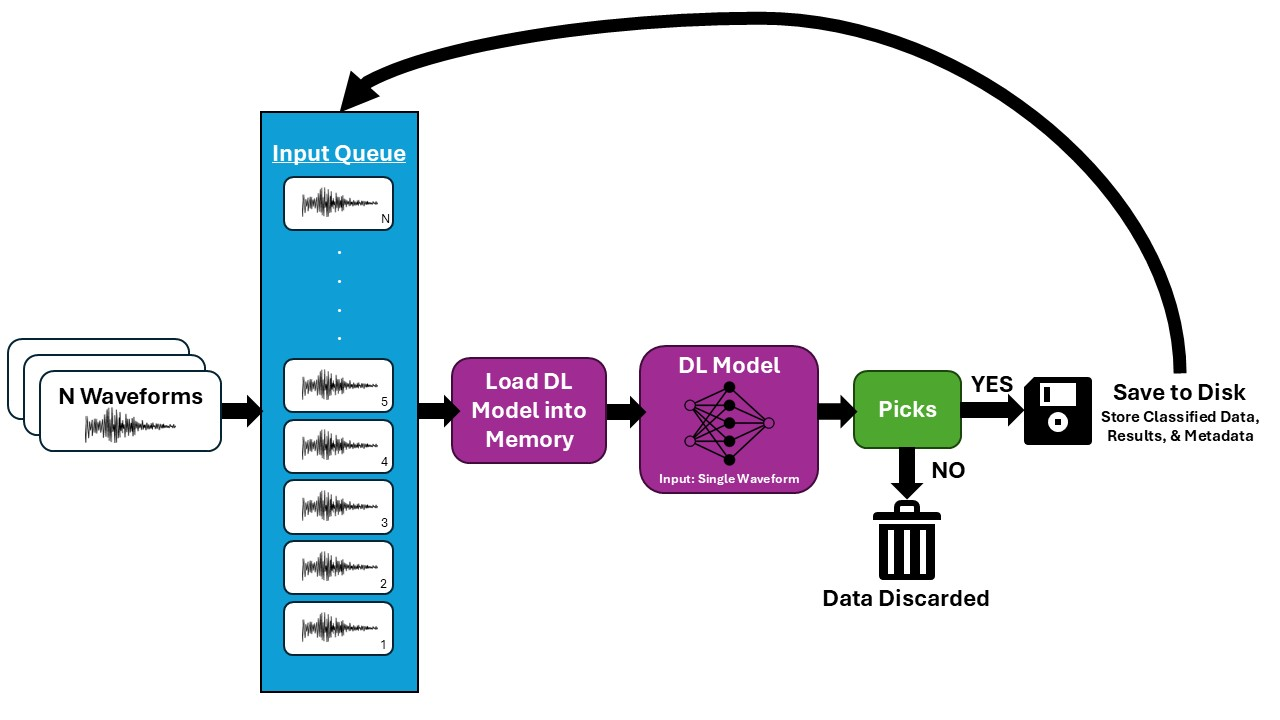
\includegraphics[width=0.92\linewidth]{figures/fig1.JPG}
\caption*{Figure 1. Serial baseline workflow. Waveforms are processed sequentially by a single DL model instance. Each waveform must wait for the previous one to complete, creating a linear bottleneck that scales poorly with network size.}
\end{figure}

\clearpage
\begin{figure}[H]
\centering
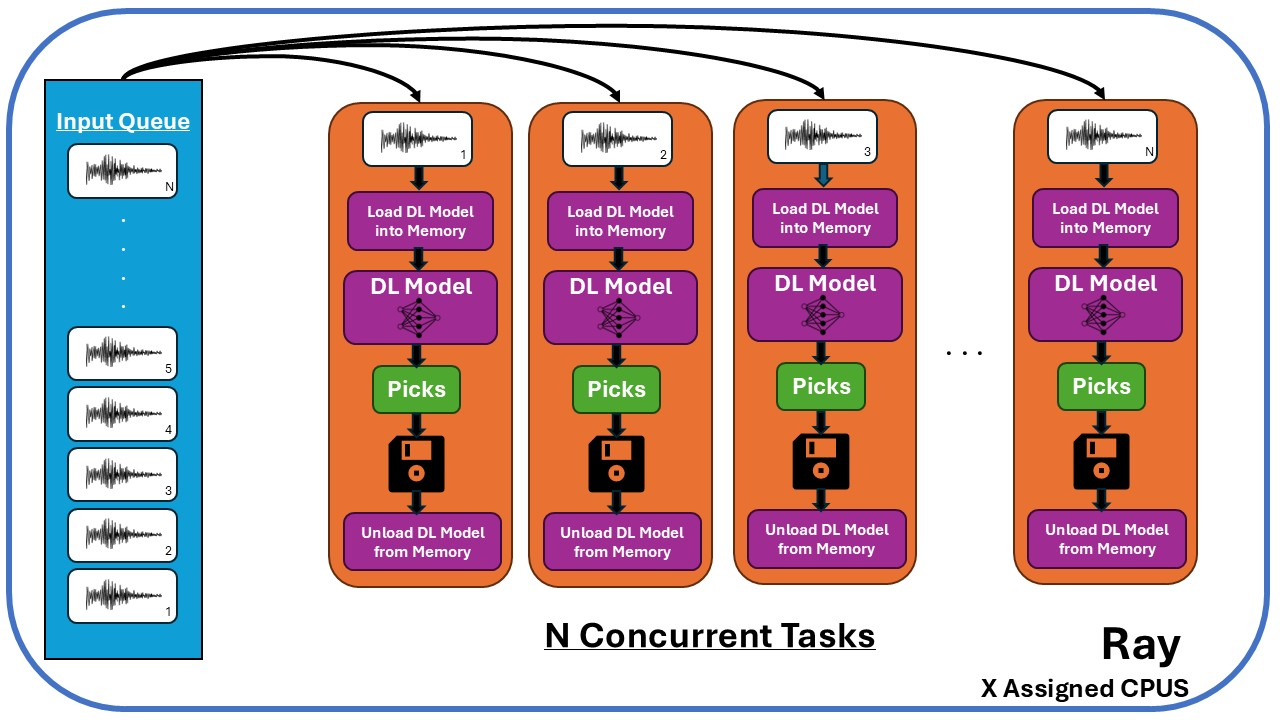
\includegraphics[width=0.92\linewidth]{figures/fig2.JPG}
\caption*{Figure 2. Ripper workflow. Each task independently loads the model, performs inference, and unloads. Multiple tasks run in parallel but incur repeated framework initialization overhead per station.}
\end{figure}

\clearpage
\begin{figure}[H]
\centering
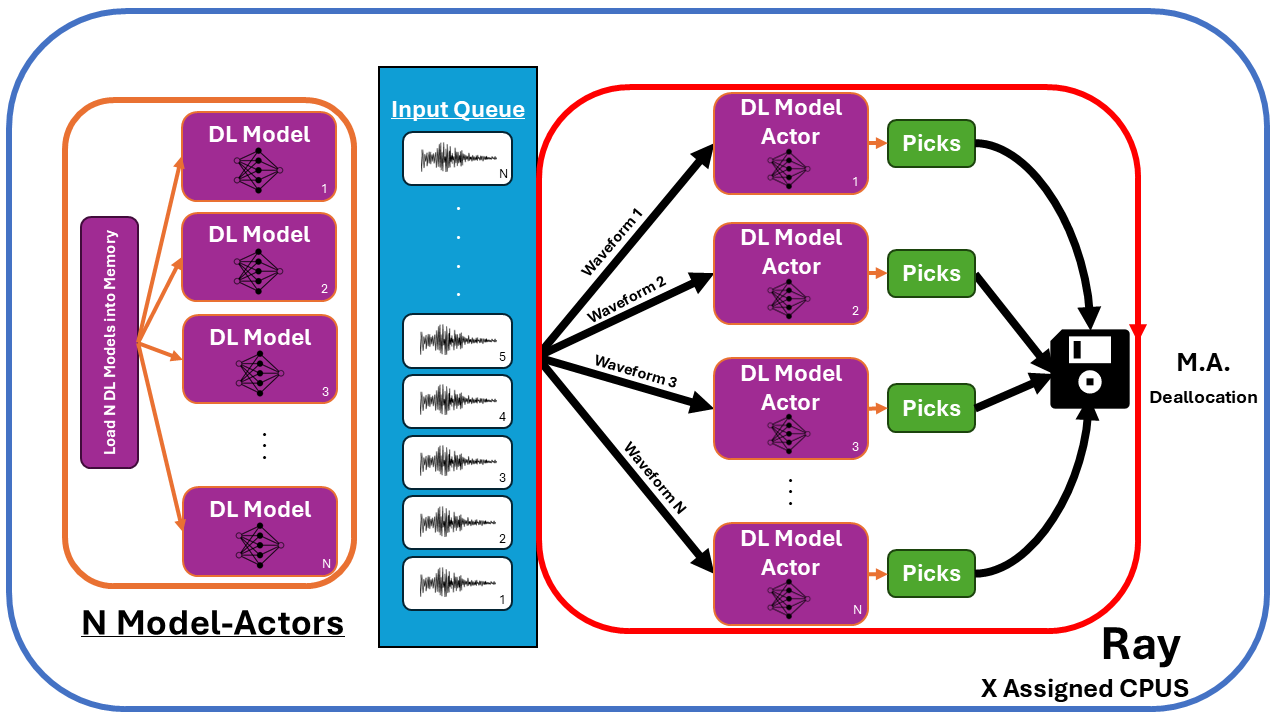
\includegraphics[width=0.92\linewidth]{figures/fig3.PNG}
\caption*{Figure 3. Model-Actor workflow. Persistent inference actors maintain loaded models in memory (or GPU VRAM). Waveforms are dispatched to actors as a stream, eliminating load/unload overhead and maximizing throughput.}
\end{figure}

\clearpage
\begin{figure}[H]
\centering
\rotatebox{90}{%
  \begin{minipage}{0.85\textheight}
    \centering
    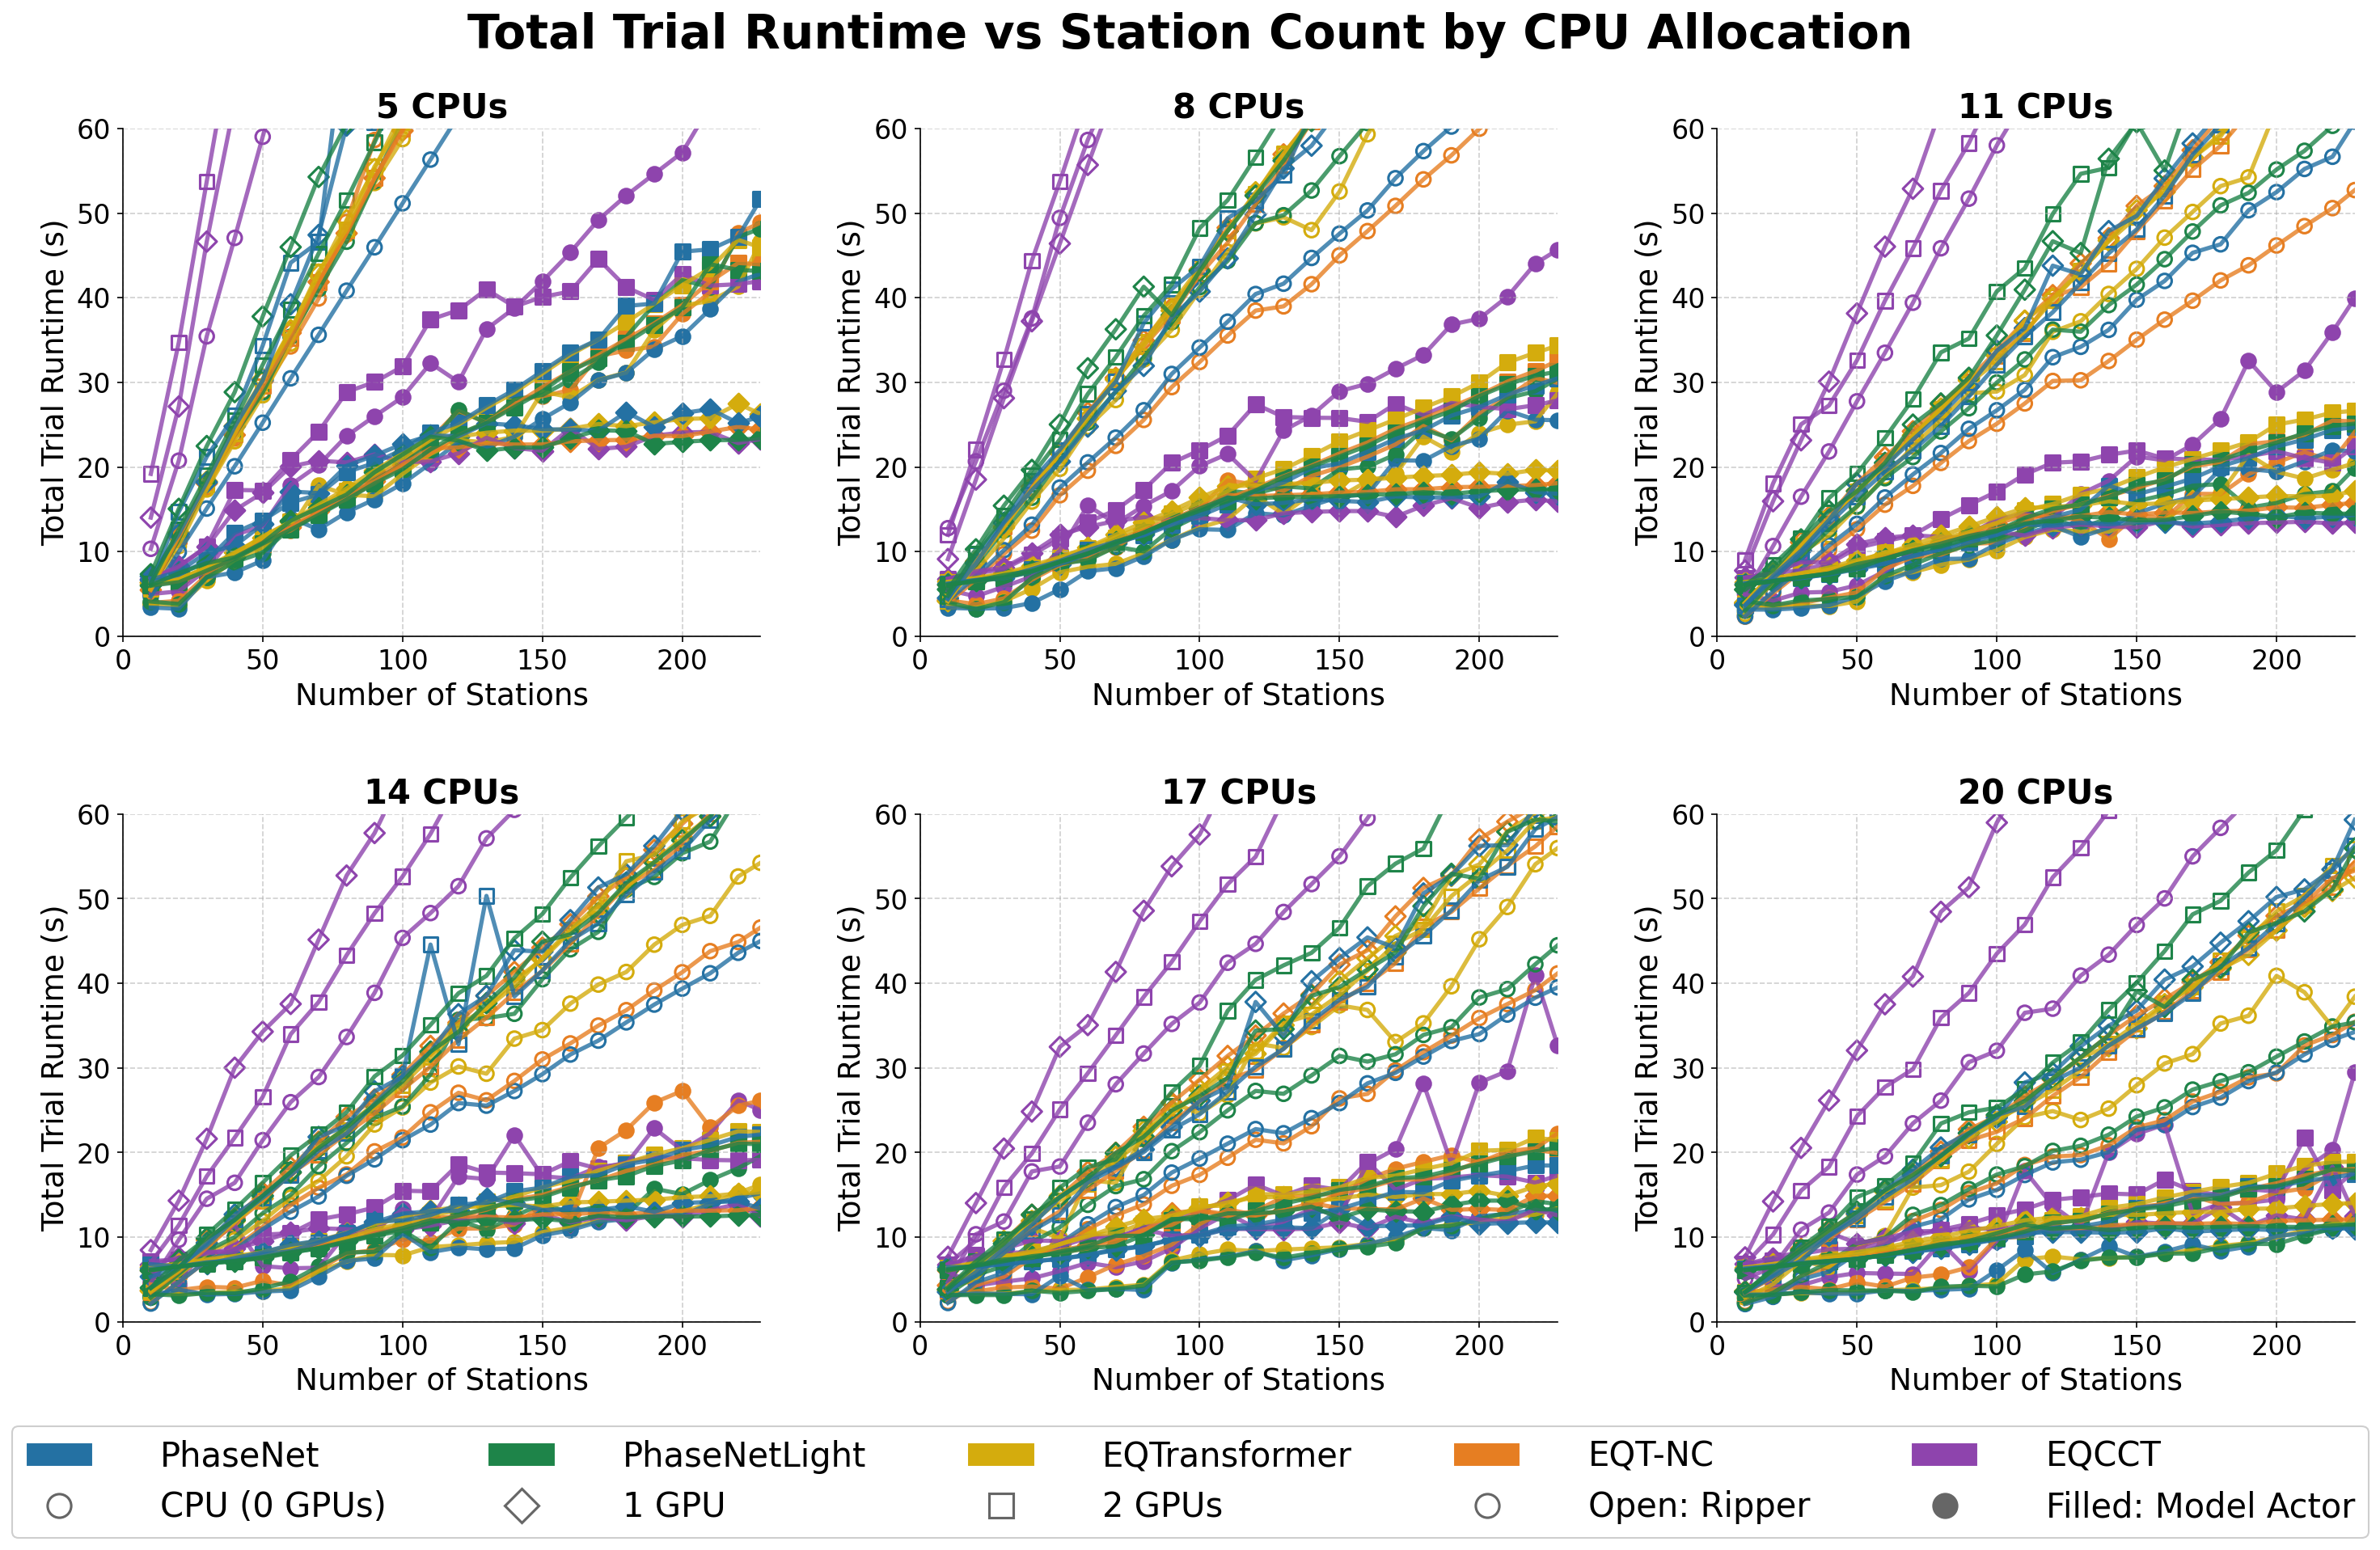
\includegraphics[width=\linewidth]{figures/fig4_runtime_3d.png}
    \caption*{Figure 4. Comparison of total trial runtime across all models and parallelization methods. Data points are plotted every 10 stations from 10 to 228. Fig.~5 and Table~4 summarize best 228-station totals.}
  \end{minipage}%
}
\end{figure}

\clearpage
\begin{figure}[H]
\centering
\rotatebox{90}{%
  \begin{minipage}{0.85\textheight}
    \centering
    
\includegraphics[width=\linewidth]{figures/fig5.png}
    \caption*{Figure 5. Minimum total runtime at 228 stations for Ripper versus Model-Actor (left: CPU, right: GPU). Bars are best successful end-to-end times at 228 stations per strategy. Dashed red line: 30~s target.}
  \end{minipage}%
}
\end{figure}

\clearpage
\begin{figure}[H]
\centering
\rotatebox{90}{%
  \begin{minipage}{0.85\textheight}
    \centering
    
\includegraphics[width=\linewidth]{figures/fig6.png}
    \caption*{Figure 6. Peak process-tree RAM (CPU) and VRAM (GPU) from the load-only benchmark: all $N$ workers held resident while sampling; bars show the maximum over 25~s samples (1.25~s interval). $N$ from best 228-station trial rows; R = Ripper tasks, MA = actors.}
  \end{minipage}%
}
\end{figure}

\clearpage
\begin{figure}[H]
\centering
\rotatebox{90}{%
  \begin{minipage}{0.85\textheight}
    \centering
    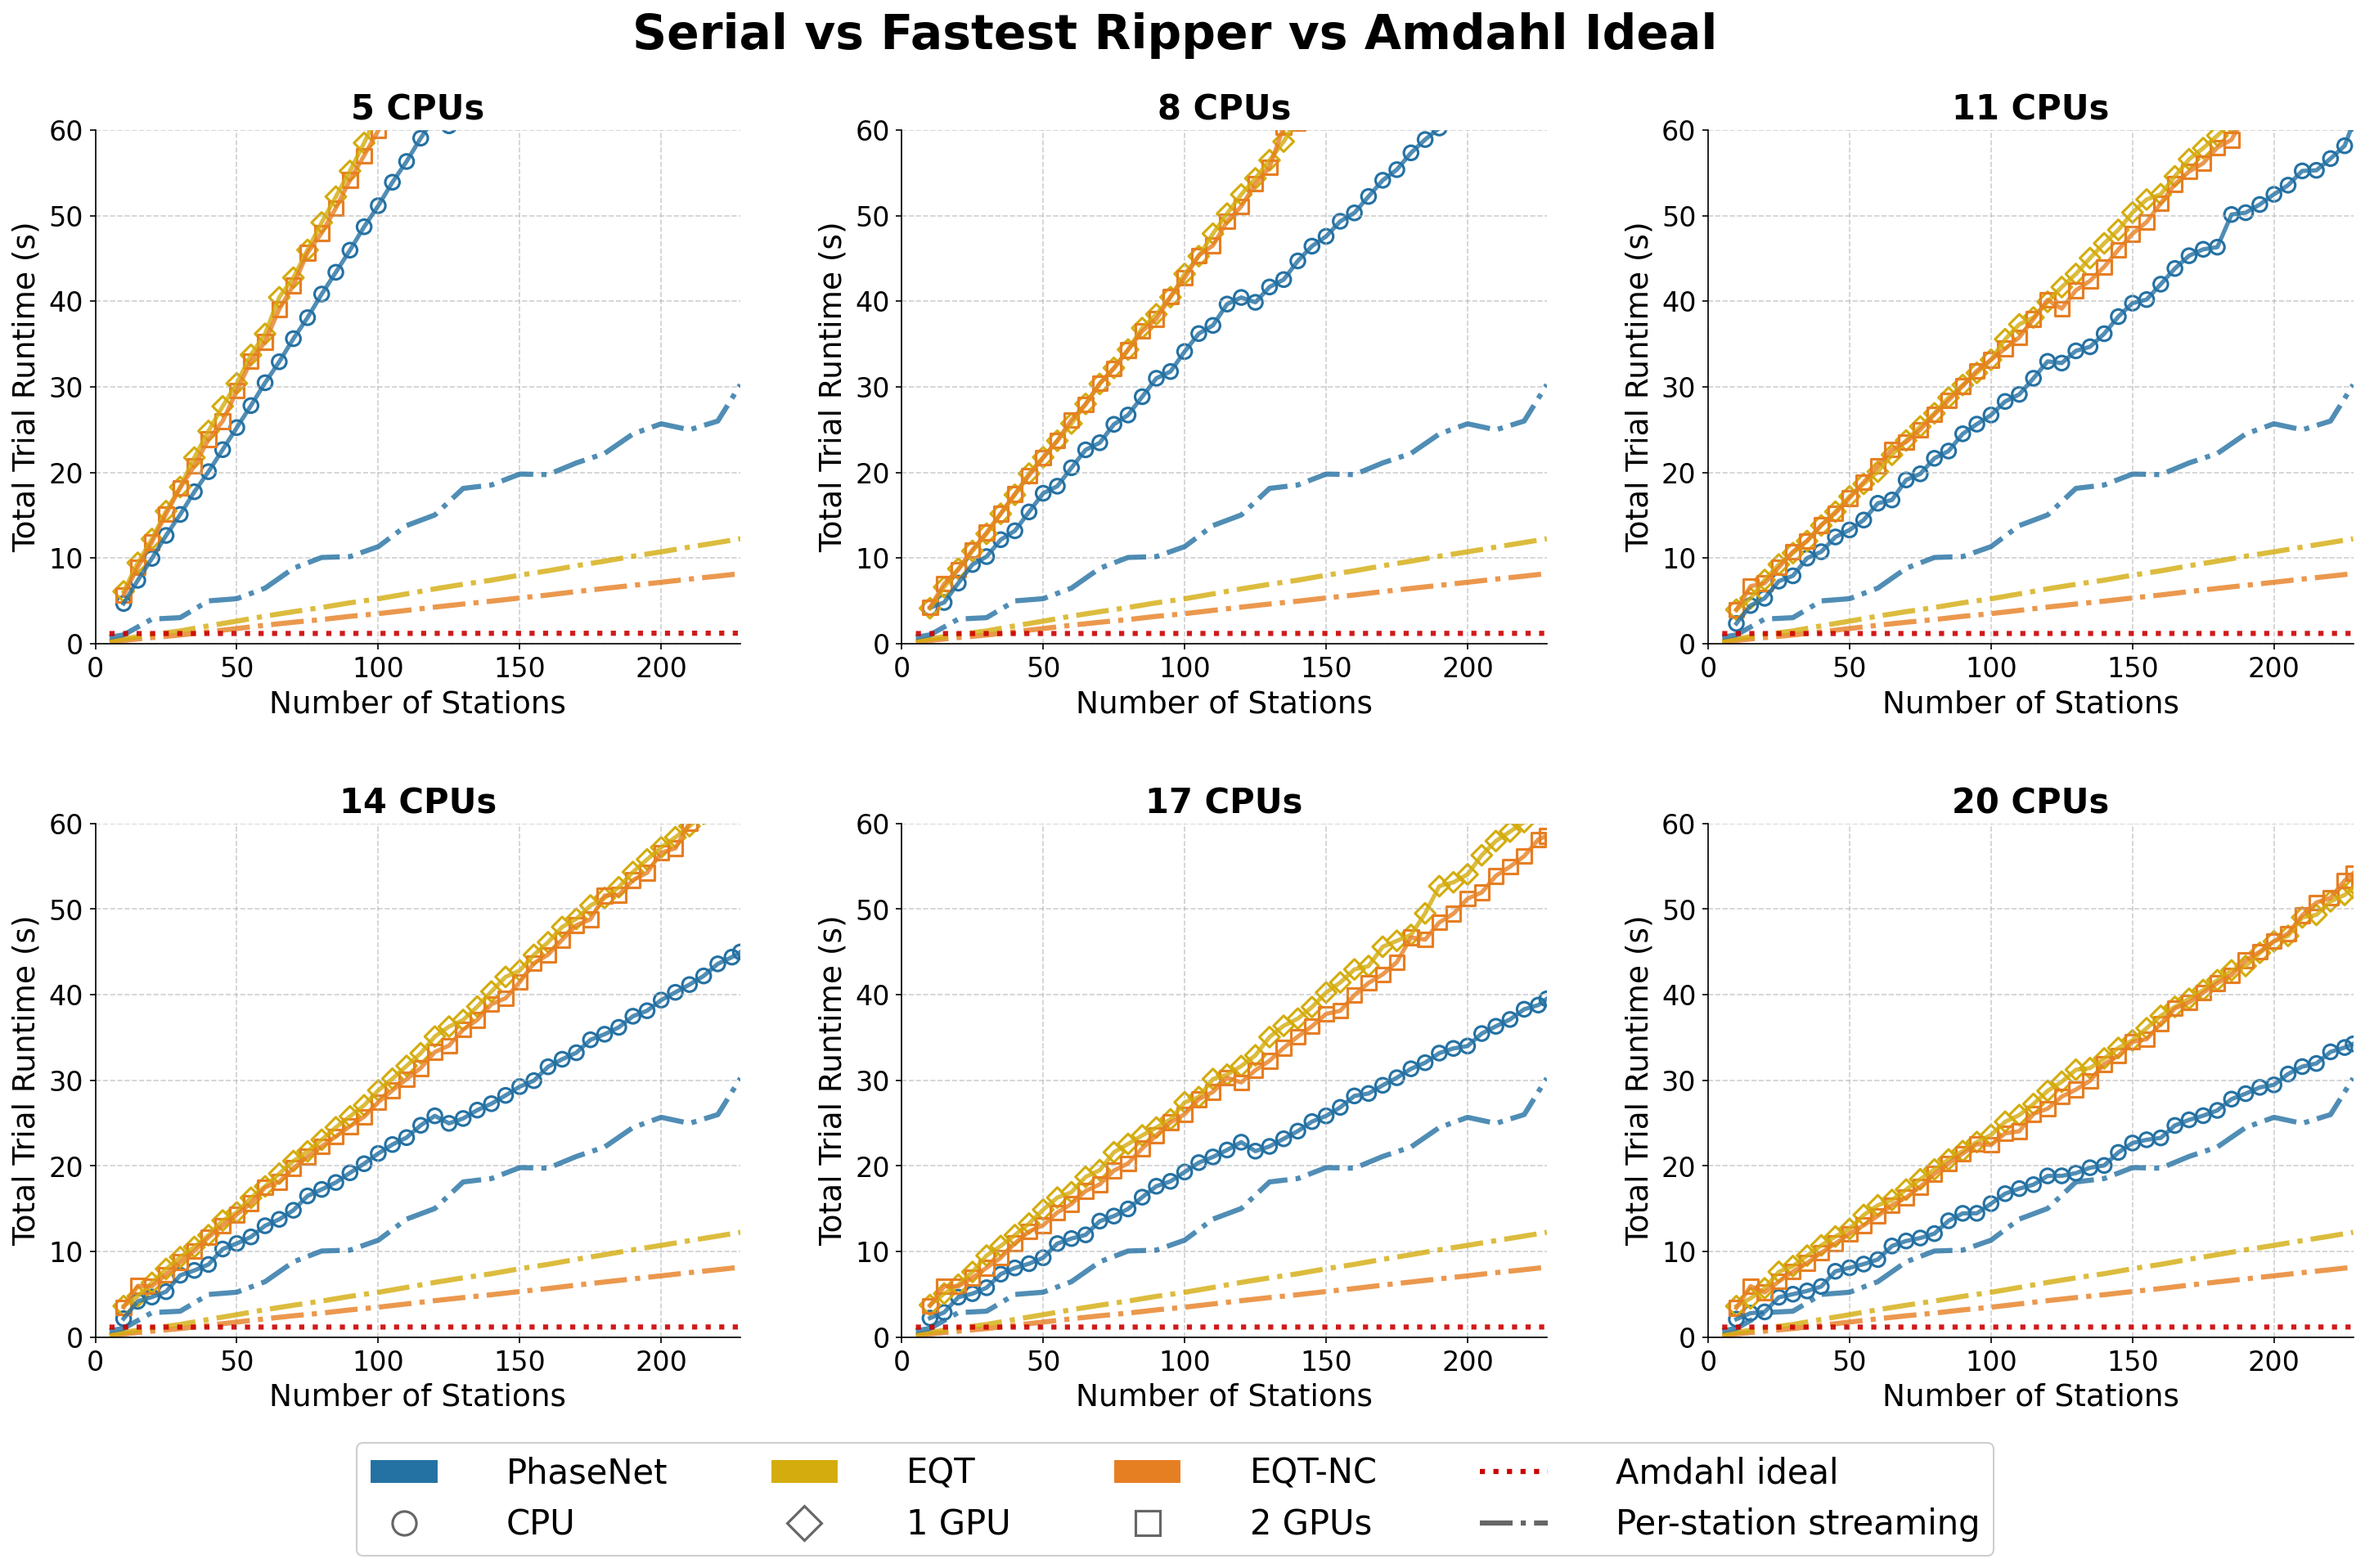
\includegraphics[width=\linewidth]{figures/fig7_serial_vs_ripper.png}
    \caption*{Figure 7. Serial baseline versus fastest Ripper configurations, with the batch-based Amdahl reference shown for each CPU allocation. For each Ripper hardware class, a single model is selected from the tested pool based on the lowest \emph{mean} total runtime across successful trials; this model defines the Ripper curve in each panel. Serial curves use the CPU spot-check grid in Table~2 (interpolated between anchors). The figure emphasizes scaling with network size rather than the individual minima reported in Table~4.}
  \end{minipage}%
}
\end{figure}

\clearpage
\begin{figure}[H]
\centering
\rotatebox{90}{%
  \begin{minipage}{0.85\textheight}
    \centering
    
\includegraphics[width=\linewidth]{figures/fig8_serial_vs_modelactor.png}
    \caption*{Figure 8. Serial baselines versus fastest Model-Actor configurations, with the Amdahl ideal limit shown for each CPU allocation. As in Figure 7, a single model is selected based on the lowest \emph{mean} total runtime across successful trials; this model defines the Model-Actor curve in each panel. Serial curves use the CPU spot-check grid in Table~2. The red dotted line denotes the Amdahl ideal, representing the theoretical minimum runtime under perfectly scalable batch processing.}
  \end{minipage}%
}
\end{figure}

\clearpage
\begin{landscape}

\begin{center}
\textbf{Table 1.} Single-process SeisBench baselines: load (minimum over five fresh load cycles), merged-stream \texttt{annotate()} on all \(N\) stations, and sequential \texttt{classify()} (mean wall time per station = total classify time divided by \(N\)). All times in seconds.

\vspace{0.8em}
\small
\begin{tabular}{lccccccc}
\toprule
\textbf{Model} & \textbf{Device} & \textbf{CPUs} & \textbf{GPUs} & \textbf{\(N\)} & \textbf{Load} & \textbf{Ann.} & \textbf{Cls./stn} \\
\midrule
PhaseNet       & CPU & 1 & 0 & 228 & 1.206 & 0.317 & 0.261 \\
PhaseNet       & GPU & 1 & 1 & 228 & 1.186 & 0.206 & 0.011 \\
PhaseNet       & CPU & 1 & 0 & 250 & 1.206 & 3.965 & 0.841 \\
PhaseNet       & GPU & 1 & 1 & 250 & 1.238 & 0.281 & 0.011 \\
PhaseNet       & CPU & 1 & 0 & 580 & 1.194 & 0.713 & 0.226 \\
PhaseNet       & GPU & 1 & 1 & 580 & 1.217 & 0.553 & 0.011 \\
PhaseNetLight  & CPU & 1 & 0 & 228 & 1.185 & 0.267 & 0.015 \\
PhaseNetLight  & GPU & 1 & 1 & 228 & 1.178 & 0.199 & 0.006 \\
PhaseNetLight  & CPU & 1 & 0 & 250 & 1.198 & 3.121 & 0.009 \\
PhaseNetLight  & GPU & 1 & 1 & 250 & 1.198 & 0.222 & 0.006 \\
PhaseNetLight  & CPU & 1 & 0 & 580 & 1.163 & 0.649 & 0.009 \\
PhaseNetLight  & GPU & 1 & 1 & 580 & 1.169 & 0.539 & 0.006 \\
EQTransformer  & CPU & 1 & 0 & 228 & 1.182 & 1.219 & 0.070 \\
EQTransformer  & GPU & 1 & 1 & 228 & 1.185 & 0.550 & 0.056 \\
EQTransformer  & CPU & 1 & 0 & 250 & 1.211 & 24.307 & 0.080 \\
EQTransformer  & GPU & 1 & 1 & 250 & 1.180 & 0.536 & 0.055 \\
EQTransformer  & CPU & 1 & 0 & 580 & 1.179 & 1.634 & 0.079 \\
EQTransformer  & GPU & 1 & 1 & 580 & 1.193 & 0.881 & 0.056 \\
EQT-NC         & CPU & 1 & 0 & 228 & 1.184 & 1.054 & 0.045 \\
EQT-NC         & GPU & 1 & 1 & 228 & 1.181 & 0.494 & 0.031 \\
EQT-NC         & CPU & 1 & 0 & 250 & 1.181 & 1.180 & 0.047 \\
EQT-NC         & GPU & 1 & 1 & 250 & 1.186 & 0.487 & 0.031 \\
EQT-NC         & CPU & 1 & 0 & 580 & 1.184 & 1.458 & 0.051 \\
EQT-NC         & GPU & 1 & 1 & 580 & 1.178 & 0.816 & 0.031 \\
\bottomrule
\end{tabular}
\end{center}

\end{landscape}

\clearpage
\begin{landscape}

\begin{center}
\textbf{Table 2.} CPU serial spot-checks (minimum over five runs per quantity). \textbf{Ann} = merged-stream \texttt{annotate()} time for all \(N\) stations; \textbf{Cls} = total sequential \texttt{classify()} time for all \(N\) stations (seconds). Load = minimum over five independent load cycles. Panel (a): TexNet 230-station subtree; (b): 250-station tree; (c): 580-station tree. These grids anchor the empirical serial curves in Figures~7--8.

\vspace{0.6em}
\scriptsize
\textbf{(a) \(N\) from 230-station dataset.}

\begin{tabular}{l r rrrrrrrrrrrr}
\toprule
\textbf{Model} & \textbf{Ld} & \multicolumn{2}{c}{\(N{=}10\)} & \multicolumn{2}{c}{\(N{=}50\)} & \multicolumn{2}{c}{\(N{=}100\)} & \multicolumn{2}{c}{\(N{=}150\)} & \multicolumn{2}{c}{\(N{=}200\)} & \multicolumn{2}{c}{\(N{=}228\)} \\
 & & Ann & Cls & Ann & Cls & Ann & Cls & Ann & Cls & Ann & Cls & Ann & Cls \\
\midrule
PhaseNet & 1.169 & 0.023 & 0.819 & 0.085 & 5.914 & 0.147 & 11.454 & 0.212 & 17.279 & 0.287 & 19.912 & 0.324 & 27.623 \\
PhaseNetLight & 1.169 & 0.020 & 0.064 & 0.068 & 0.326 & 0.143 & 0.652 & 0.185 & 0.973 & 0.229 & 1.306 & 0.265 & 1.481 \\
EQTransformer & 1.163 & 0.087 & 0.585 & 0.206 & 2.762 & 0.471 & 5.496 & 0.672 & 8.305 & 0.879 & 11.003 & 1.016 & 12.541 \\
EQT-NC & 1.163 & 0.069 & 0.386 & 0.186 & 1.796 & 0.432 & 3.568 & 0.660 & 5.437 & 0.884 & 7.302 & 1.011 & 8.302 \\
\bottomrule
\end{tabular}

\vspace{1em}
\textbf{(b) \(N\) from 250-station dataset.}

\begin{tabular}{l r rrrrrrrrrrrrr}
\toprule
\textbf{Model} & \textbf{Ld} & \multicolumn{2}{c}{\(N{=}10\)} & \multicolumn{2}{c}{\(N{=}50\)} & \multicolumn{2}{c}{\(N{=}100\)} & \multicolumn{2}{c}{\(N{=}150\)} & \multicolumn{2}{c}{\(N{=}200\)} & \multicolumn{2}{c}{\(N{=}228\)} & \multicolumn{2}{c}{\(N{=}250\)} \\
 & & Ann & Cls & Ann & Cls & Ann & Cls & Ann & Cls & Ann & Cls & Ann & Cls & Ann & Cls \\
\midrule
PhaseNet & 1.175 & 0.019 & 1.125 & 0.066 & 6.108 & 0.142 & 12.321 & 0.194 & 18.014 & 0.244 & 24.590 & 0.289 & 25.883 & 0.324 & 31.498 \\
PhaseNetLight & 1.181 & 0.017 & 0.064 & 0.061 & 0.323 & 0.125 & 0.650 & 0.170 & 0.975 & 0.226 & 1.294 & 0.262 & 1.477 & 0.290 & 1.619 \\
EQTransformer & 1.178 & 0.080 & 0.581 & 0.158 & 2.609 & 0.371 & 5.410 & 0.631 & 8.188 & 0.779 & 10.955 & 0.960 & 12.528 & 1.014 & 13.740 \\
EQT-NC & 1.157 & 0.059 & 0.384 & 0.137 & 1.746 & 0.348 & 3.611 & 0.606 & 5.441 & 0.821 & 7.298 & 0.912 & 8.342 & 1.011 & 9.151 \\
\bottomrule
\end{tabular}

\vspace{1em}
\textbf{(c) \(N\) from 580-station dataset.}

\begin{tabular}{l r rrrrrrrrrrrrrrr}
\toprule
\textbf{Model} & \textbf{Ld} & \multicolumn{2}{c}{\(N{=}10\)} & \multicolumn{2}{c}{\(N{=}50\)} & \multicolumn{2}{c}{\(N{=}100\)} & \multicolumn{2}{c}{\(N{=}150\)} & \multicolumn{2}{c}{\(N{=}200\)} & \multicolumn{2}{c}{\(N{=}228\)} & \multicolumn{2}{c}{\(N{=}250\)} & \multicolumn{2}{c}{\(N{=}580\)} \\
 & & Ann & Cls & Ann & Cls & Ann & Cls & Ann & Cls & Ann & Cls & Ann & Cls & Ann & Cls & Ann & Cls \\
\midrule
PhaseNet & 1.158 & 0.020 & 0.797 & 0.063 & 5.738 & 0.114 & 11.293 & 0.163 & 17.230 & 0.228 & 22.941 & 0.266 & 27.778 & 0.283 & 30.640 & 0.634 & 67.109 \\
PhaseNetLight & 1.165 & 0.018 & 0.063 & 0.059 & 0.319 & 0.108 & 0.637 & 0.153 & 0.963 & 0.214 & 1.287 & 0.243 & 1.461 & 0.265 & 1.600 & 0.589 & 3.736 \\
EQTransformer & 1.143 & 0.075 & 0.595 & 0.155 & 2.872 & 0.213 & 5.493 & 0.302 & 9.314 & 0.432 & 11.276 & 0.481 & 12.696 & 0.518 & 13.912 & 1.316 & 32.663 \\
EQT-NC & 1.171 & 0.057 & 0.379 & 0.117 & 1.886 & 0.189 & 3.503 & 0.288 & 5.479 & 0.410 & 7.382 & 0.483 & 8.291 & 0.479 & 9.111 & 1.274 & 21.449 \\
\bottomrule
\end{tabular}
\end{center}

\end{landscape}

\clearpage
\begin{landscape}

\begin{center}
\textbf{Table 3.} Per-instance memory budgets (MB) used by RAPID to cap concurrency and avoid out-of-memory errors.

\vspace{1em}
\small
\begin{tabular}{llccccccc}
\toprule
\textbf{Model} & \textbf{Framework} & \multicolumn{2}{c}{\textbf{Host RAM -- CPU (MB)}} & \multicolumn{2}{c}{\textbf{Host RAM -- GPU (MB)}} & \multicolumn{3}{c}{\textbf{GPU VRAM (MB)}} \\
\cmidrule(lr){3-4} \cmidrule(lr){5-6} \cmidrule(lr){7-9}
 & & Base & Per Ripper/Actor & Base & Per Ripper/Actor & Base & Per Ripper & Per Actor \\
\midrule
PhaseNet      & PyTorch    & 502  & 2,038 & 870  & 2,406 & 500  & 850  & 1,524 \\
PhaseNetLight & PyTorch    & 502  & 2,038 & 861  & 2,397 & 500  & 850  & 1,524 \\
EQTransformer & PyTorch    & 521  & 2,057 & 1,001 & 2,537 & 528  & 1,056 & 1,552 \\
EQT-NC        & PyTorch    & 524  & 2,060 & 1,017 & 2,553 & 530  & 1,060 & 1,554 \\
EQCCT         & TensorFlow & 728  & 2,264 & 2,311 & 3,847 & 1,732 & 3,464 & 2,756 \\
\bottomrule
\end{tabular}
\end{center}

\end{landscape}

\clearpage
\begin{landscape}

\begin{center}
\textbf{Table 4.} Best successful Ripper total time at 228 stations, sorted by fastest time. CPU rows are minima over Ray CPUs tested; GPU rows report the best one-GPU and two-GPU Ripper totals separately.

\vspace{0.8em}
\small
\begin{tabular}{lccccc}
\toprule
\textbf{Model} & \textbf{Device} & \textbf{CPUs} & \textbf{GPUs} & \textbf{Conc. Tasks} & \textbf{Ripper Picking/Total (s)} \\
\midrule
PhaseNet         & CPU & 20 & 0 & 91  & 34.25 \\
PhaseNetLight    & CPU & 20 & 0 & 91  & 35.38 \\
EQTransformer-NC & CPU & 20 & 0 & 228 & 35.45 \\
EQTransformer    & CPU & 20 & 0 & 137 & 38.42 \\
EQTransformer    & GPU & 20 & 1 & 22  & 52.48 \\
EQTransformer-NC & GPU & 20 & 1 & 22  & 53.31 \\
EQTransformer-NC & GPU & 20 & 2 & 44  & 54.17 \\
EQTransformer    & GPU & 20 & 2 & 44  & 55.88 \\
PhaseNetLight    & GPU & 20 & 1 & 22  & 55.95 \\
PhaseNet         & GPU & 20 & 2 & 44  & 56.27 \\
PhaseNet         & GPU & 20 & 1 & 22  & 59.32 \\
PhaseNetLight    & GPU & 20 & 2 & 44  & 67.61 \\
EQCCT            & CPU & 20 & 0 & 137 & 76.07 \\
EQCCT            & GPU & 20 & 2 & 24  & 96.10 \\
EQCCT            & GPU & 20 & 1 & 12  & 127.35 \\
\bottomrule
\end{tabular}
\end{center}

\end{landscape}

\clearpage
\begin{landscape}

\begin{center}
\textbf{Table 5.} Best successful Model-Actor total time at 228 stations, sorted by fastest time. CPU rows are minima over Ray CPUs tested; GPU rows report the best one-GPU and two-GPU Model-Actor totals separately. Setup OH is actor-creation (or equivalent) setup time as a percentage of total Model-Actor trial time.

\vspace{1em}
\small
\begin{tabular}{lcccccccc}
\toprule
\textbf{Model} & \textbf{Device} & \textbf{CPUs} & \textbf{GPUs} & \textbf{Actors} & \textbf{Setup (s)} & \textbf{Pick (s)} & \textbf{Total (s)} & \textbf{Setup OH} \\
\midrule
PhaseNet      & GPU & 20 & 1 & 22 & 6.70  & 4.27 & 10.97 & 61.0\% \\
PhaseNetLight & CPU & 20 & 0 & 46 & 7.04  & 4.28 & 11.47 & 61.4\% \\
PhaseNet      & CPU & 20 & 0 & 46 & 7.21  & 4.16 & 11.48 & 62.8\% \\
PhaseNetLight & GPU & 20 & 1 & 22 & 6.96  & 4.56 & 11.53 & 60.4\% \\
EQTransformer & CPU & 20 & 0 & 46 & 6.92  & 4.70 & 11.63 & 59.5\% \\
EQT-NC        & GPU & 20 & 1 & 22 & 6.91  & 5.19 & 12.11 & 57.1\% \\
EQCCT         & GPU & 14 & 1 & 12 & 4.64  & 7.82 & 12.47 & 37.2\% \\
EQTransformer & GPU & 20 & 1 & 22 & 7.12  & 6.92 & 14.05 & 50.7\% \\
EQCCT         & GPU & 17 & 2 & 24 & 7.95  & 9.33 & 17.29 & 46.0\% \\
PhaseNet      & GPU & 20 & 2 & 44 & 10.88 & 6.60 & 17.49 & 62.2\% \\
EQT-NC        & CPU & 20 & 0 & 46 & 12.88 & 4.70 & 17.74 & 72.6\% \\
PhaseNetLight & GPU & 20 & 2 & 44 & 10.83 & 7.02 & 17.86 & 60.6\% \\
EQT-NC        & GPU & 20 & 2 & 44 & 10.75 & 7.30 & 18.06 & 59.5\% \\
EQTransformer & GPU & 20 & 2 & 44 & 10.76 & 8.16 & 18.93 & 56.9\% \\
EQCCT         & CPU & 14 & 0 & 46 & 12.73 & 12.23 & 25.01 & 50.9\% \\
\bottomrule
\end{tabular}
\end{center}

\end{landscape}

\clearpage
\begin{landscape}

\begin{center}
\textbf{Table 6.} Memory utilization for each Model-Actor row in Table~5. All memory values are in MB.

\vspace{1em}
\small
\begin{tabular}{lccccccccc}
\toprule
\textbf{Model} & \textbf{Device} & \textbf{CPUs} & \textbf{GPUs} & \textbf{Actors} & \textbf{Req. RAM} & \textbf{Tree RAM} & \textbf{Req. VRAM} & \textbf{Tree VRAM} & \textbf{Peak RAM} \\
\midrule
PhaseNet      & GPU & 20 & 1 & 22 & 58,564  & 32,813 & 36,344 & 11,580 & 782 \\
PhaseNetLight & CPU & 20 & 0 & 46 & 105,524 & 49,017 & 0      & 0      & 273 \\
PhaseNet      & CPU & 20 & 0 & 46 & 105,524 & 51,694 & 0      & 0      & 274 \\
PhaseNetLight & GPU & 20 & 1 & 22 & 58,366  & 39,068 & 36,344 & 11,580 & 280 \\
EQTransformer & CPU & 20 & 0 & 46 & 106,398 & 51,012 & 0      & 0      & 258 \\
EQT-NC        & GPU & 20 & 1 & 22 & 61,798  & 43,578 & 37,004 & 12,273 & 244 \\
EQCCT         & GPU & 14 & 1 & 12 & 49,236  & 15,363 & 34,608 & 40,316 & 456 \\
EQTransformer & GPU & 20 & 1 & 22 & 61,446  & 42,982 & 36,960 & 12,226 & 275 \\
EQCCT         & GPU & 17 & 2 & 24 & 98,472  & 18,506 & 69,216 & 43,675 & 958 \\
PhaseNet      & GPU & 20 & 2 & 44 & 117,128 & 59,490 & 72,688 & 526    & 1,084 \\
EQT-NC        & CPU & 20 & 0 & 46 & 106,536 & 56,537 & 0      & 0      & 200 \\
PhaseNetLight & GPU & 20 & 2 & 44 & 116,732 & 72,936 & 72,688 & 23,161 & 383 \\
EQT-NC        & GPU & 20 & 2 & 44 & 123,596 & 82,457 & 74,008 & 24,545 & 378 \\
EQTransformer & GPU & 20 & 2 & 44 & 122,892 & 80,613 & 73,920 & 24,453 & 398 \\
EQCCT         & CPU & 14 & 0 & 46 & 115,920 & 48,701 & 0      & 0      & 202 \\
\bottomrule
\end{tabular}
\end{center}

\end{landscape}


\end{document}
